% Options for packages loaded elsewhere
% Options for packages loaded elsewhere
\PassOptionsToPackage{unicode}{hyperref}
\PassOptionsToPackage{hyphens}{url}
%
\documentclass[
  ignorenonframetext,
  aspectratio=169,
  russian,
]{beamer}
\newif\ifbibliography
\usepackage{pgfpages}
\setbeamertemplate{caption}[numbered]
\setbeamertemplate{caption label separator}{: }
\setbeamercolor{caption name}{fg=normal text.fg}
\beamertemplatenavigationsymbolshorizontal
% remove section numbering
\setbeamertemplate{part page}{
  \centering
  \begin{beamercolorbox}[sep=16pt,center]{part title}
    \usebeamerfont{part title}\insertpart\par
  \end{beamercolorbox}
}
\setbeamertemplate{section page}{
  \centering
  \begin{beamercolorbox}[sep=12pt,center]{section title}
    \usebeamerfont{section title}\insertsection\par
  \end{beamercolorbox}
}
\setbeamertemplate{subsection page}{
  \centering
  \begin{beamercolorbox}[sep=8pt,center]{subsection title}
    \usebeamerfont{subsection title}\insertsubsection\par
  \end{beamercolorbox}
}
% Prevent slide breaks in the middle of a paragraph
\widowpenalties 1 10000
\raggedbottom
\AtBeginPart{
  \frame{\partpage}
}
\AtBeginSection{
  \ifbibliography
  \else
    \frame{\sectionpage}
  \fi
}
\AtBeginSubsection{
  \frame{\subsectionpage}
}
\usepackage{iftex}
\ifPDFTeX
  \usepackage[T1]{fontenc}
  \usepackage[utf8]{inputenc}
  \usepackage{textcomp} % provide euro and other symbols
\else % if luatex or xetex
  \usepackage{unicode-math} % this also loads fontspec
  \defaultfontfeatures{Scale=MatchLowercase}
  \defaultfontfeatures[\rmfamily]{Ligatures=TeX,Scale=1}
\fi
\usepackage{lmodern}

\ifPDFTeX\else
  % xetex/luatex font selection
\fi
% Use upquote if available, for straight quotes in verbatim environments
\IfFileExists{upquote.sty}{\usepackage{upquote}}{}
\IfFileExists{microtype.sty}{% use microtype if available
  \usepackage[]{microtype}
  \UseMicrotypeSet[protrusion]{basicmath} % disable protrusion for tt fonts
}{}


\usepackage{longtable,booktabs,array}
\usepackage{calc} % for calculating minipage widths
\usepackage{caption}
% Make caption package work with longtable
\makeatletter
\def\fnum@table{\tablename~\thetable}
\makeatother
\usepackage{graphicx}
\makeatletter
\newsavebox\pandoc@box
\newcommand*\pandocbounded[1]{% scales image to fit in text height/width
  \sbox\pandoc@box{#1}%
  \Gscale@div\@tempa{\textheight}{\dimexpr\ht\pandoc@box+\dp\pandoc@box\relax}%
  \Gscale@div\@tempb{\linewidth}{\wd\pandoc@box}%
  \ifdim\@tempb\p@<\@tempa\p@\let\@tempa\@tempb\fi% select the smaller of both
  \ifdim\@tempa\p@<\p@\scalebox{\@tempa}{\usebox\pandoc@box}%
  \else\usebox{\pandoc@box}%
  \fi%
}
% Set default figure placement to htbp
\def\fps@figure{htbp}
\makeatother



\ifLuaTeX
\usepackage[bidi=basic,provide=*]{babel}
\else
\usepackage[bidi=default,provide=*]{babel}
\fi
% get rid of language-specific shorthands (see #6817):
\let\LanguageShortHands\languageshorthands
\def\languageshorthands#1{}


\setlength{\emergencystretch}{3em} % prevent overfull lines

\providecommand{\tightlist}{%
  \setlength{\itemsep}{0pt}\setlength{\parskip}{0pt}}



 

\usepackage[]{csquotes}

\IfFileExists{plex-otf.sty}{
  %% Full TeXlive
  % \usepackage[%
  %   % math,
  %   RM={Scale=0.94},SS={Scale=0.94},SScon={Scale=0.94},TT={Scale=MatchLowercase,FakeStretch=0.9},DefaultFeatures={Ligatures=Common}
  % ]{plex-otf}
}{
  %% TinyTeX
  \usepackage{libertine}
}

%%% Load theme
% https://deic.uab.cat/~iblanes/beamer_gallery/
\IfFileExists{beamerthemegotham.sty}{
  %% Full TeXlive
  \usetheme{gotham}
  \gothamset{
    numbering=totalpagenumber,
    parttocframe default=off,
    sectiontocframe default=off,
    subsectiontocframe default=off,
  }
}{
  %% TinyTeX
  \usetheme{Madrid}
}
\makeatletter
\@ifpackageloaded{caption}{}{\usepackage{caption}}
\AtBeginDocument{%
\ifdefined\contentsname
  \renewcommand*\contentsname{Содержание}
\else
  \newcommand\contentsname{Содержание}
\fi
\ifdefined\listfigurename
  \renewcommand*\listfigurename{Список иллюстраций}
\else
  \newcommand\listfigurename{Список иллюстраций}
\fi
\ifdefined\listtablename
  \renewcommand*\listtablename{Список таблиц}
\else
  \newcommand\listtablename{Список таблиц}
\fi
\ifdefined\figurename
  \renewcommand*\figurename{Рисунок}
\else
  \newcommand\figurename{Рисунок}
\fi
\ifdefined\tablename
  \renewcommand*\tablename{Таблица}
\else
  \newcommand\tablename{Таблица}
\fi
}
\@ifpackageloaded{float}{}{\usepackage{float}}
\floatstyle{ruled}
\@ifundefined{c@chapter}{\newfloat{codelisting}{h}{lop}}{\newfloat{codelisting}{h}{lop}[chapter]}
\floatname{codelisting}{Список}
\newcommand*\listoflistings{\listof{codelisting}{Листинги}}
\makeatother
\makeatletter
\makeatother
\makeatletter
\@ifpackageloaded{caption}{}{\usepackage{caption}}
\@ifpackageloaded{subcaption}{}{\usepackage{subcaption}}
\makeatother

\usepackage{bookmark}
\IfFileExists{xurl.sty}{\usepackage{xurl}}{} % add URL line breaks if available
\urlstyle{same}
\hypersetup{
  pdftitle={Лабораторная работа 7},
  pdfauthor={Сидорова Александра Андреевна},
  pdflang={ru-RU},
  hidelinks,
  pdfcreator={LaTeX via pandoc}}


\title{Лабораторная работа 7}
\subtitle{НБИбд-01-25}
\author{Сидорова Александра Андреевна}
\date{}

\begin{document}
\frame{\titlepage}

\renewcommand*\contentsname{Содержание}
\begin{frame}[allowframebreaks]
  \frametitle{Содержание}
  \setcounter{tocdepth}{1}
  \tableofcontents
\end{frame}
\setcounter{tocdepth}{1}
\tableofcontents
}

\begin{frame}{Докладчик}
\phantomsection\label{ux434ux43eux43aux43bux430ux434ux447ux438ux43a}
\begin{itemize}[<+->]
\tightlist
\item
  Сидорова Александра Андреевна
\item
  ученица
\item
  1 курс Бизнес-информатика
\item
  Российский университет дружбы народов им. П. Лумумбы
\item
  НБИбд-01-25
\item
  \url{https://github.com/aasidorova1/study_2025-2026_os-intro}
\end{itemize}

::: ::: \{.column width=\enquote{30\%}\}

\pandocbounded{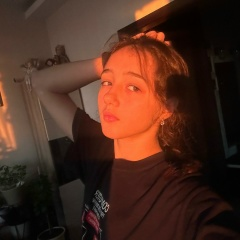
\includegraphics[keepaspectratio]{./image/111.jpg}}

::: ::::::::::::::
\end{frame}

\section{Вводная
часть}\label{ux432ux432ux43eux434ux43dux430ux44f-ux447ux430ux441ux442ux44c}

\begin{frame}{Вводная часть}
В этой презентации я представлю мою 7 лабораторную работу связанную с
файловой системой Linux.
\end{frame}

\begin{frame}{Актуальность}
\phantomsection\label{ux430ux43aux442ux443ux430ux43bux44cux43dux43eux441ux442ux44c}
\begin{itemize}[<+->]
\tightlist
\item
  умение пользоватьс файловой системой Linux необходимо студенту
\item
  приобретение рактических навыков по применению команд для работы с
  файлами и каталогами способстувет развитию студента по направлению
\item
  тренируются навыки в работе с Linux
\end{itemize}
\end{frame}

\begin{frame}{Объект и предмет исследования}
\phantomsection\label{ux43eux431ux44aux435ux43aux442-ux438-ux43fux440ux435ux434ux43cux435ux442-ux438ux441ux441ux43bux435ux434ux43eux432ux430ux43dux438ux44f}
\begin{itemize}[<+->]
\tightlist
\item
  файловая система Linux
\item
  работа с файлами и каталогами
\item
  использование диска и обслуживанию файловой системы
\end{itemize}
\end{frame}

\begin{frame}{Цели и задачи}
\phantomsection\label{ux446ux435ux43bux438-ux438-ux437ux430ux434ux430ux447ux438}
Ознакомление с файловой системой Linux, её структурой, именами и
содержанием каталогов. Приобретение практических навыков по применению
команд для работы с файлами и каталогами, по управлению процессами (и
работами), по проверке исполь- зования диска и обслуживанию файловой
системы.
\end{frame}

\section{Задание}\label{ux437ux430ux434ux430ux43dux438ux435}

\begin{frame}{Задание}
\begin{enumerate}[<+->]
\tightlist
\item
  Выполните все примеры, приведённые в первой части описания
  лабораторной работы.
\item
  Выполните следующие действия, зафиксировав в отчёте по лабораторной
  работе используемые при этом команды и результаты их выполнения,
  результаты вы увидете дальше
\end{enumerate}
\end{frame}

\section{Теоретическое
введение}\label{ux442ux435ux43eux440ux435ux442ux438ux447ux435ux441ux43aux43eux435-ux432ux432ux435ux434ux435ux43dux438ux435}

\begin{frame}{1.Команды для работы с файлами и каталогами}
\phantomsection\label{ux43aux43eux43cux430ux43dux434ux44b-ux434ux43bux44f-ux440ux430ux431ux43eux442ux44b-ux441-ux444ux430ux439ux43bux430ux43cux438-ux438-ux43aux430ux442ux430ux43bux43eux433ux430ux43cux438}
-\enquote{touch имя-файла} -\enquote{cat имя-файла} -\enquote{less
имя-файла}
\end{frame}

\begin{frame}{2.Копирование файлов и каталогов}
\phantomsection\label{ux43aux43eux43fux438ux440ux43eux432ux430ux43dux438ux435-ux444ux430ux439ux43bux43eux432-ux438-ux43aux430ux442ux430ux43bux43eux433ux43eux432}
-\enquote{cp {[}-опции{]} исходный\_файл целевой\_файл}
\end{frame}

\begin{frame}{3.Перемещение и переименование файлов и каталогов}
\phantomsection\label{ux43fux435ux440ux435ux43cux435ux449ux435ux43dux438ux435-ux438-ux43fux435ux440ux435ux438ux43cux435ux43dux43eux432ux430ux43dux438ux435-ux444ux430ux439ux43bux43eux432-ux438-ux43aux430ux442ux430ux43bux43eux433ux43eux432}
-\enquote{mv {[}-опции{]} старый\_файл новый\_файл}
\end{frame}

\begin{frame}{4.Права доступа}
\phantomsection\label{ux43fux440ux430ux432ux430-ux434ux43eux441ux442ux443ux43fux430}
\begin{longtable}[]{@{}
  >{\raggedright\arraybackslash}p{(\linewidth - 6\tabcolsep) * \real{0.1111}}
  >{\raggedright\arraybackslash}p{(\linewidth - 6\tabcolsep) * \real{0.1212}}
  >{\raggedright\arraybackslash}p{(\linewidth - 6\tabcolsep) * \real{0.0707}}
  >{\raggedright\arraybackslash}p{(\linewidth - 6\tabcolsep) * \real{0.6970}}@{}}
\toprule\noalign{}
\begin{minipage}[b]{\linewidth}\raggedright
Право
\end{minipage} & \begin{minipage}[b]{\linewidth}\raggedright
Обозначение
\end{minipage} & \begin{minipage}[b]{\linewidth}\raggedright
Файл
\end{minipage} & \begin{minipage}[b]{\linewidth}\raggedright
Каталог
\end{minipage} \\
\midrule\noalign{}
\endhead
Чтение & \enquote*{r} & Разрешены просмотр и копирование & Разрешён
просмотр списка входящих файлов \\
Запись & \enquote*{w} & Разрешены изменение и переименование & Разрешены
создание и удаление файлов \\
Выполнение & \enquote*{x} & Разрешено выполнение файла (скриптов и/или
программ) & Разрешён доступ в каталог и есть возможность сделать его
текущим \\
\bottomrule\noalign{}
\end{longtable}
\end{frame}

\begin{frame}{5.Изменение прав доступа}
\phantomsection\label{ux438ux437ux43cux435ux43dux435ux43dux438ux435-ux43fux440ux430ux432-ux434ux43eux441ux442ux443ux43fux430}
\enquote{chmod режим имя\_файла}
\end{frame}

\section{Выполнение лабораторной
работы}\label{ux432ux44bux43fux43eux43bux43dux435ux43dux438ux435-ux43bux430ux431ux43eux440ux430ux442ux43eux440ux43dux43eux439-ux440ux430ux431ux43eux442ux44b}

\begin{frame}{Выполнение лабораторной работы}
\begin{block}{Слайд 1}
\phantomsection\label{ux441ux43bux430ux439ux434-1}
Выполняю все примеры приведенные в первой части работы. В начале я с
помощью команды less просмтариваю файл text.txt по странично (до этого
создала его с помощью команды touch). Потом с помощью команды cat
просматриваю тотже файл. После жтого захожу в католог лабораторной 2 и с
помощью команды head просматриваю первые 4 строки файла. (рис.1)

\begin{figure}[H]

{\centering \pandocbounded{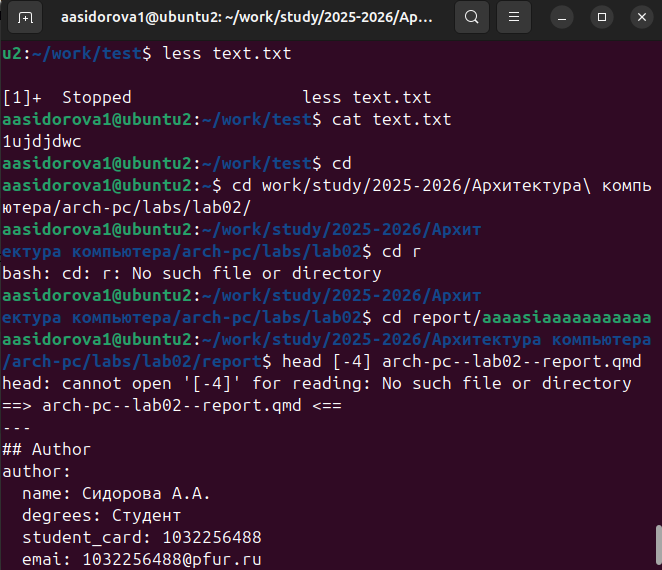
\includegraphics[keepaspectratio]{image/l7.01.png}}

}

\caption{рис.1}

\end{figure}%
\end{block}

\begin{block}{Слайд 2}
\phantomsection\label{ux441ux43bux430ux439ux434-2}
Потом с помощью команды tail просматриваю посление 6 строчек этого же
файла. (рис.2)

\begin{figure}[H]

{\centering \pandocbounded{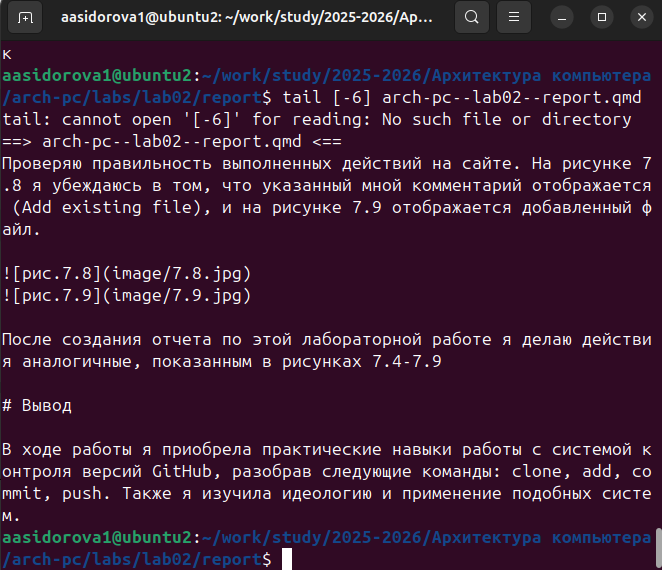
\includegraphics[keepaspectratio]{image/l7.02.png}}

}

\caption{рис.2}

\end{figure}%
\end{block}

\begin{block}{Слайд 3}
\phantomsection\label{ux441ux43bux430ux439ux434-3}
Перехожу в свой тестовый каталог, который был создан заранее. В нем я
создаю файл abc1, потом копирую этот файл в файл april и его же копирую
в may. Создаю директорию monthly. Копирую april и may в monthly. (рис.3)

\begin{figure}[H]

{\centering \pandocbounded{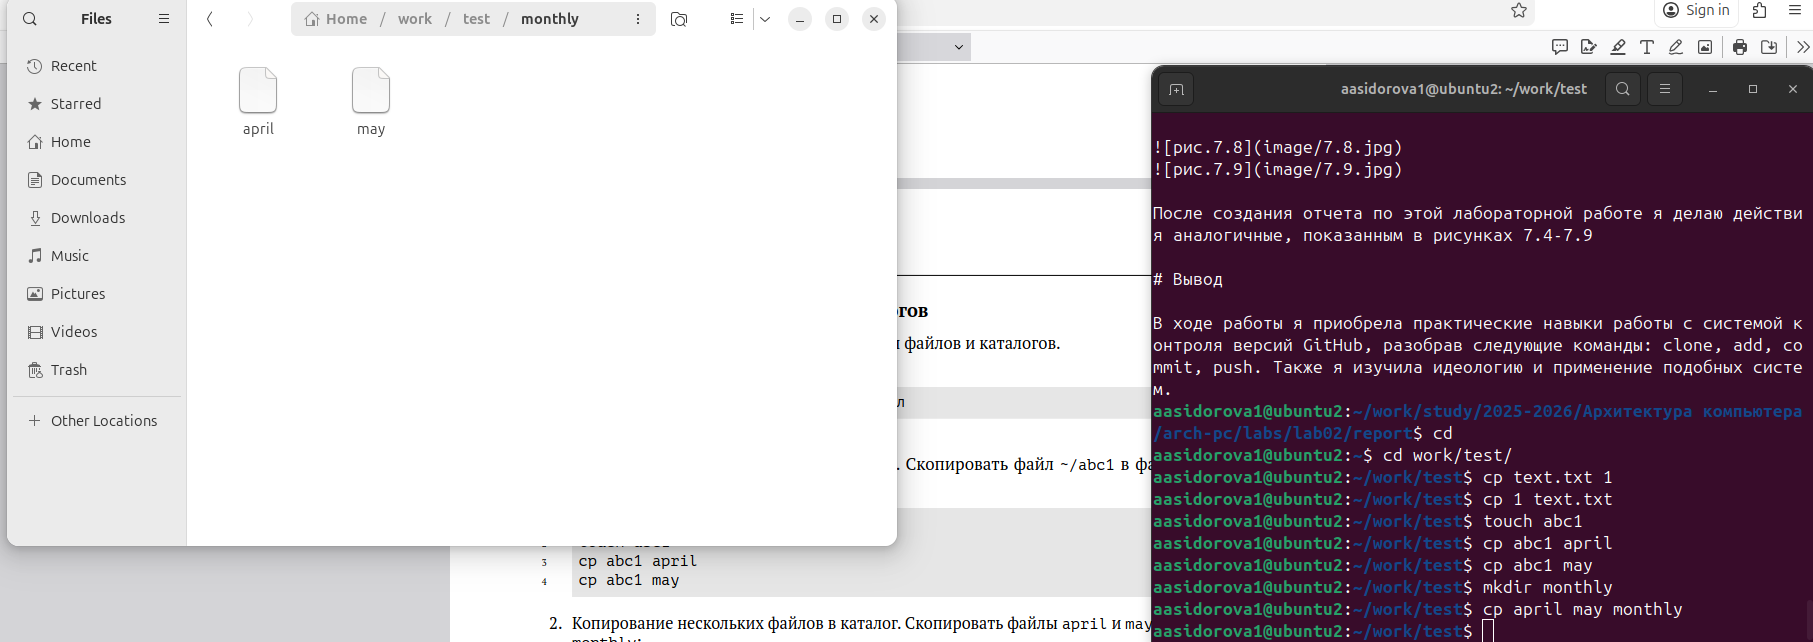
\includegraphics[keepaspectratio]{image/l7.05.png}}

}

\caption{рис.3}

\end{figure}%
\end{block}

\begin{block}{Слайд 4}
\phantomsection\label{ux441ux43bux430ux439ux434-4}
Копирую файл monthly/may в файл с именем june и проверяю (рис.4)

\begin{figure}[H]

{\centering \pandocbounded{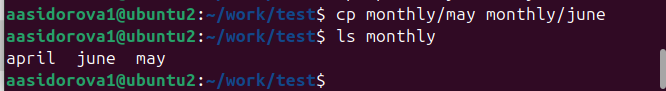
\includegraphics[keepaspectratio]{image/l7.06.png}}

}

\caption{рис.4}

\end{figure}%
\end{block}

\begin{block}{Слайд 5}
\phantomsection\label{ux441ux43bux430ux439ux434-5}
Создаю директрию monthly.00. Копирую каталог monthly в каталог
monthly.00. Копирую каталог monthly.00 в каталог /tmp (рис.5)

\begin{figure}[H]

{\centering \pandocbounded{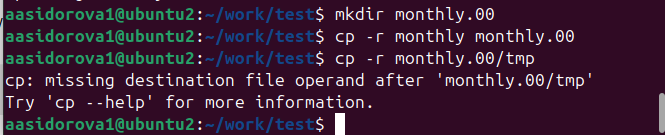
\includegraphics[keepaspectratio]{image/l7.07.png}}

}

\caption{рис.5}

\end{figure}%
\end{block}

\begin{block}{Слайд 6}
\phantomsection\label{ux441ux43bux430ux439ux434-6}
Изменяю название файла april на july в домашнем каталоге. Перемещаю файл
july в каталог monthly.00. (рис.6)

\begin{figure}[H]

{\centering \pandocbounded{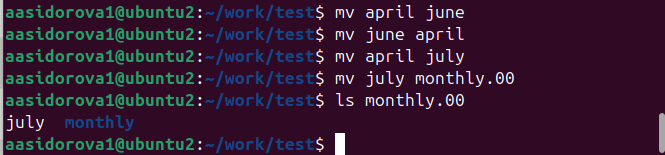
\includegraphics[keepaspectratio]{image/l7.08.png}}

}

\caption{рис.6}

\end{figure}%
\end{block}

\begin{block}{Слайд 7}
\phantomsection\label{ux441ux43bux430ux439ux434-7}
Переименовываю каталог monthly.00 в monthly.01. Перемещаю каталог
monthly.01в каталог reports. Переименовываю каталог reports/monthly.01 в
reports/monthly. (рис.7)

\begin{figure}[H]

{\centering \pandocbounded{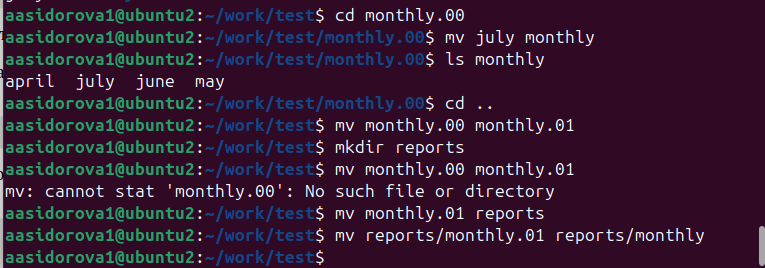
\includegraphics[keepaspectratio]{image/l7.09.png}}

}

\caption{рис.7}

\end{figure}%
\end{block}

\begin{block}{Слайд 8}
\phantomsection\label{ux441ux43bux430ux439ux434-8}
Создаю файл \textasciitilde/may с правом выполнения для владельца и
проверяю. (рис.8)

\begin{figure}[H]

{\centering \pandocbounded{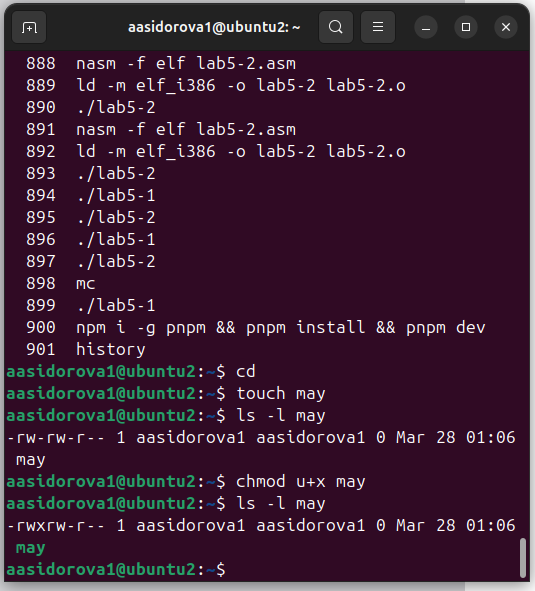
\includegraphics[keepaspectratio]{image/l71.png}}

}

\caption{рис.8}

\end{figure}%
\end{block}

\begin{block}{Слайд 9}
\phantomsection\label{ux441ux43bux430ux439ux434-9}
Лишаю владельца файла \textasciitilde/may права на выполнение. Создаю
каталог monthly с запретом на чтение для членов группы и всех остальных
пользователей (на скрине не получилось, потом исправила с помощью
числовых значаний). (рис.9)

\begin{figure}[H]

{\centering \pandocbounded{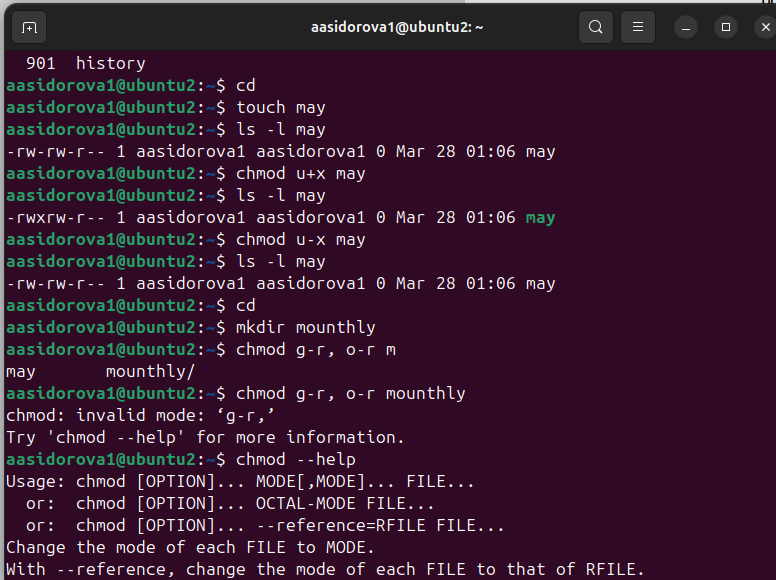
\includegraphics[keepaspectratio]{image/l72.png}}

}

\caption{рис.9}

\end{figure}%
\end{block}

\begin{block}{Слайд 10}
\phantomsection\label{ux441ux43bux430ux439ux434-10}
Создаю файл \textasciitilde/abc1 с правом записи для членов группы.
(рис.10)

\begin{figure}[H]

{\centering \pandocbounded{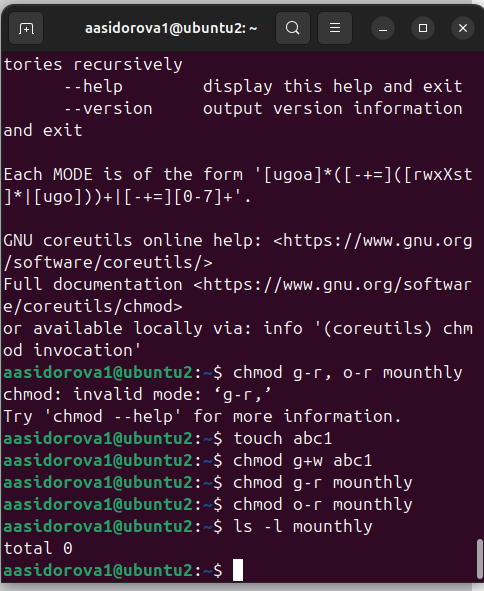
\includegraphics[keepaspectratio]{image/l73.png}}

}

\caption{рис.10}

\end{figure}%
\end{block}

\begin{block}{Слайд 11}
\phantomsection\label{ux441ux43bux430ux439ux434-11}
Использую команду mount, cat, df, fsck. (рис.11-13)

\begin{figure}[H]

{\centering \pandocbounded{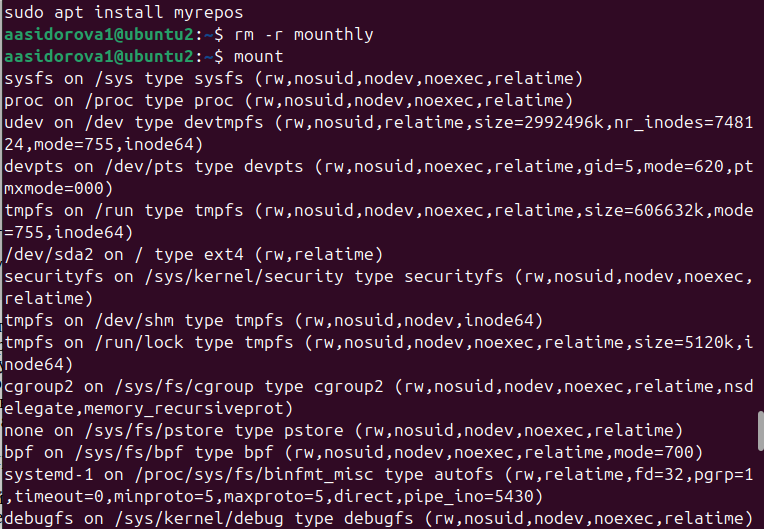
\includegraphics[keepaspectratio]{image/l74.png}}

}

\caption{рис.11}

\end{figure}%

\begin{figure}[H]

{\centering \pandocbounded{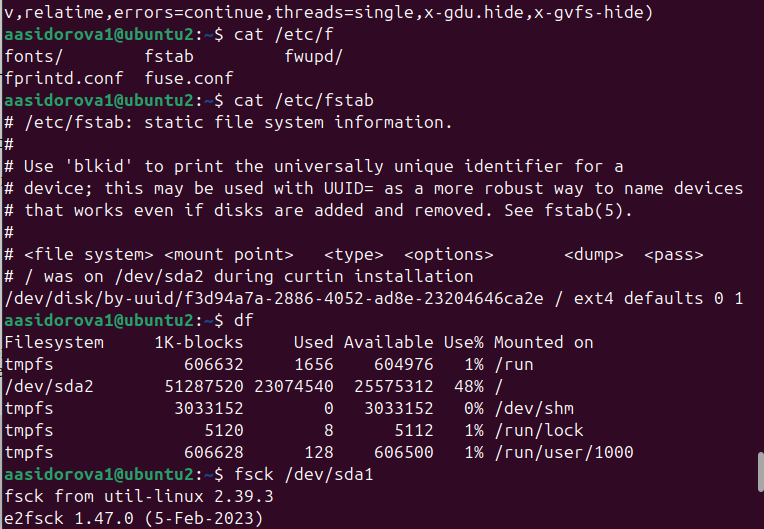
\includegraphics[keepaspectratio]{image/l75.png}}

}

\caption{рис.12}

\end{figure}%

\begin{figure}[H]

{\centering \pandocbounded{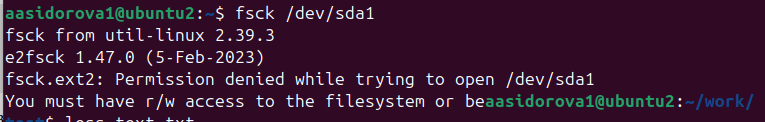
\includegraphics[keepaspectratio]{image/l76.png}}

}

\caption{рис.13}

\end{figure}%
\end{block}

\begin{block}{Выполнение лабораторной}
\phantomsection\label{ux432ux44bux43fux43eux43bux43dux435ux43dux438ux435-ux43bux430ux431ux43eux440ux430ux442ux43eux440ux43dux43eux439}
Выполнение рабораторной работы пункт 2.1. Скопировала файл
/usr/include/sound/sof/abi.h в домашний каталог и назвала его equipment.
2.2 в домашнем каталоге создала директорию ski.plases. 2.3 переместила
файл equipment в каталог \textasciitilde/ski.plases. 2.4 переименовала
файл \textasciitilde/ski.plases/equipment в
\textasciitilde/ski.plases/equiplist. 2.5 создала в домашнем каталоге
файл abc1 и скопировала его в каталог \textasciitilde/ski.plases,
назвала его equiplist2. (рис.14)

\begin{figure}[H]

{\centering \pandocbounded{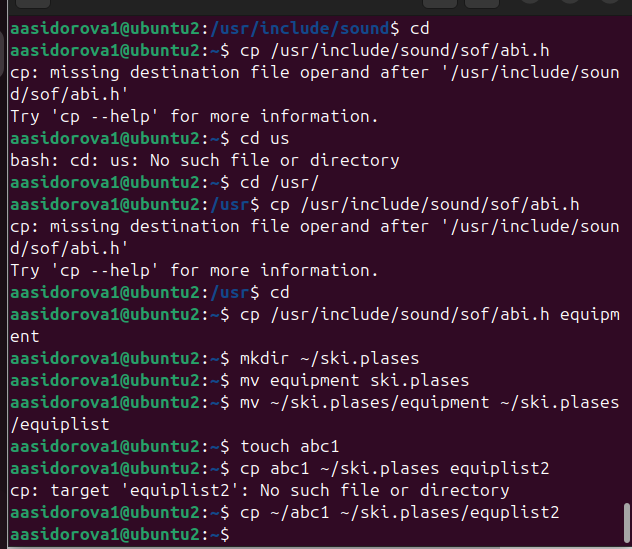
\includegraphics[keepaspectratio]{image/l77.png}}

}

\caption{рис.14}

\end{figure}%
\end{block}

\begin{block}{Выполнение лабораторной}
\phantomsection\label{ux432ux44bux43fux43eux43bux43dux435ux43dux438ux435-ux43bux430ux431ux43eux440ux430ux442ux43eux440ux43dux43eux439-1}
2.7 Перемещаю файлы \textasciitilde/ski.plases/equiplist и equiplist2 в
каталог \textasciitilde/ski.plases/equipment. 2.8 Создаю и перемещаю
каталог \textasciitilde/newdir в каталог \textasciitilde/ski.plases и
назовите его plans. (рис.15)

\begin{figure}[H]

{\centering \pandocbounded{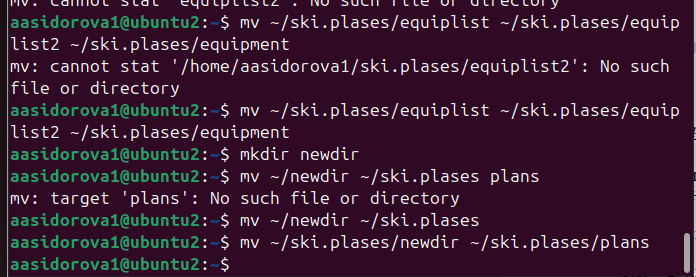
\includegraphics[keepaspectratio]{image/l78.png}}

}

\caption{рис.15}

\end{figure}%
\end{block}

\begin{block}{Выполнение лабораторной}
\phantomsection\label{ux432ux44bux43fux43eux43bux43dux435ux43dux438ux435-ux43bux430ux431ux43eux440ux430ux442ux43eux440ux43dux43eux439-2}
Создаю необходимые файлы australia, play,my\_os, feathers и с помощью
команды chmod передаю им необходимые права доступа. (рис.16-17)

\begin{figure}[H]

{\centering \pandocbounded{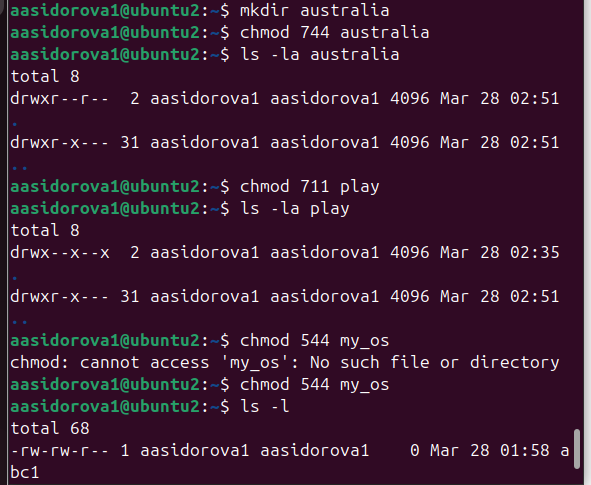
\includegraphics[keepaspectratio]{image/l79.png}}

}

\caption{рис.16}

\end{figure}%

\begin{figure}[H]

{\centering \pandocbounded{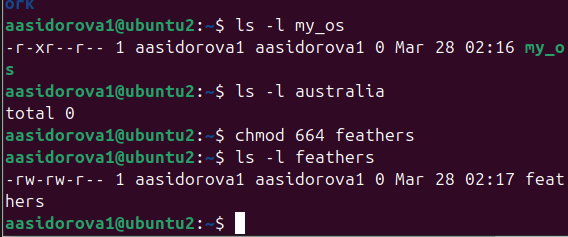
\includegraphics[keepaspectratio]{image/l710.png}}

}

\caption{рис.17}

\end{figure}%
\end{block}

\begin{block}{Выполнение лабораторной}
\phantomsection\label{ux432ux44bux43fux43eux43bux43dux435ux43dux438ux435-ux43bux430ux431ux43eux440ux430ux442ux43eux440ux43dux43eux439-3}
4.1 Просматриваю содержимое файла /etc/password с помощью cat. (рис.18)

\begin{figure}[H]

{\centering \pandocbounded{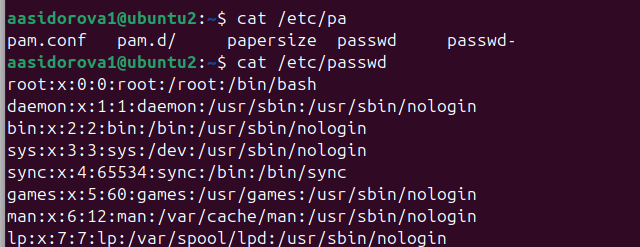
\includegraphics[keepaspectratio]{image/l711.png}}

}

\caption{рис.18}

\end{figure}%
\end{block}

\begin{block}{Выполнение лабораторной}
\phantomsection\label{ux432ux44bux43fux43eux43bux43dux435ux43dux438ux435-ux43bux430ux431ux43eux440ux430ux442ux43eux440ux43dux43eux439-4}
4.2. Скопировала файл \textasciitilde/feathers в файл
\textasciitilde/file.old. 4.3. Переместила файл \textasciitilde/file.old
в каталог \textasciitilde/play. 4.4. Скопировала каталог
\textasciitilde/play в каталог \textasciitilde/fun. 4.5. Переместила
каталог \textasciitilde/fun в каталог \textasciitilde/play и назвала его
games. 4.6. Лишила владельца файла \textasciitilde/feathers права на
чтение. 4.7. Если я попытаетесь просмотреть файл
\textasciitilde/feathers командой cat выдаст что в доступе отказано.
4.8. Если я попытаетесь скопировать файл \textasciitilde/feathers тоже в
доступе отказано. 4.9. Даю владельцу файла \textasciitilde/feathers
право на чтение. 4.10. Лишаю владельца каталога \textasciitilde/play
права на выполнение. 4.11. Перехожу в каталог \textasciitilde/play.
Пишет что в доступе отказано. 4.12. Дайте владельцу каталога
\textasciitilde/play право на выполнение. (рис.19)

\begin{figure}[H]

{\centering \pandocbounded{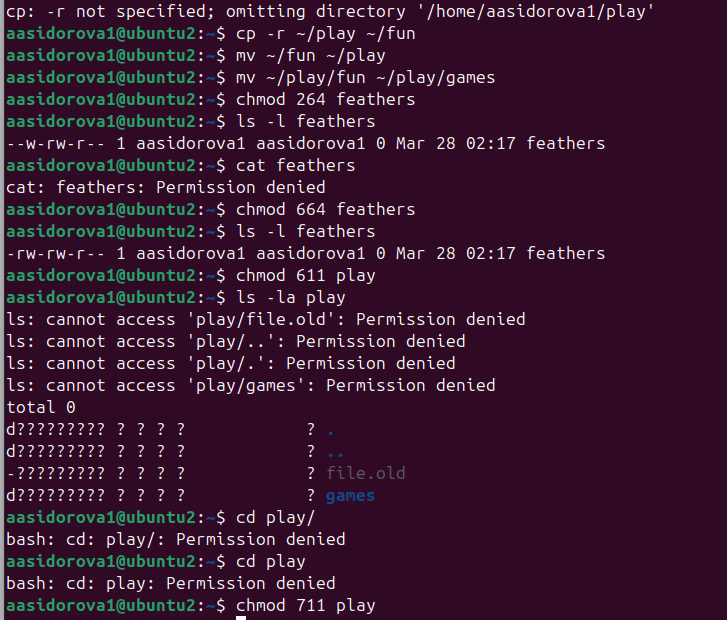
\includegraphics[keepaspectratio]{image/l712.png}}

}

\caption{рис.19}

\end{figure}%
\end{block}

\begin{block}{Выполнение лабораторной}
\phantomsection\label{ux432ux44bux43fux43eux43bux43dux435ux43dux438ux435-ux43bux430ux431ux43eux440ux430ux442ux43eux440ux43dux43eux439-5}
Читаю man по командам mount, fsck, mkfs, kill. Mount не находит файл
man. Fsck выдает информацию по использованию и по срочной помощи. Kill
выдает arguments must be process or job IDs. (рис.20)

\begin{figure}[H]

{\centering \pandocbounded{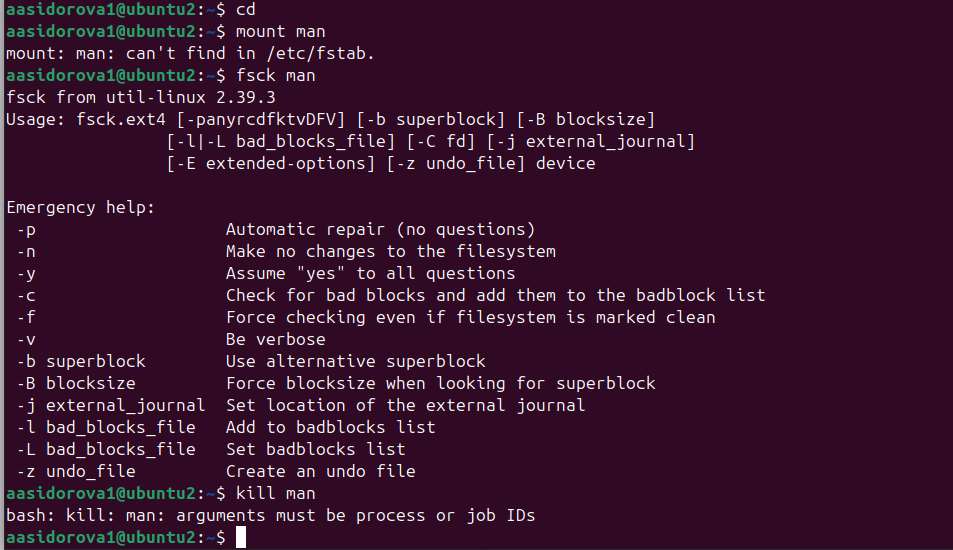
\includegraphics[keepaspectratio]{image/l713.png}}

}

\caption{рис.20}

\end{figure}%
\end{block}
\end{frame}

\section{Ответы на
вопросы}\label{ux43eux442ux432ux435ux442ux44b-ux43dux430-ux432ux43eux43fux440ux43eux441ux44b}

\begin{frame}[fragile]{Ответы на вопросы}
\begin{enumerate}[<+->]
\item
  Характеристика основных файловых систем:

  NTFS (New Technology File System): Назначение: Стандартная ФС для
  Windows NT/10/11.
\item
  / --- корневой каталог, основа всей файловой иерархии. /bin ---
  базовые исполняемые файлы для всех пользователей (ls, cp, mv и т. д.).
\end{enumerate}

\begin{verbatim}
/boot — файлы для загрузки ОС: ядро, загрузчик (GRUB), initrd.

/dev — файлы устройств (жёсткие диски, терминалы, принтеры и т. д.).

/etc — конфигурационные файлы системы и служб.

/home — домашние каталоги обычных пользователей, личные файлы и настройки.
\end{verbatim}

\begin{enumerate}[<+->]
\setcounter{enumi}{2}
\tightlist
\item
  Команда mount подключает файловую систему к определённой точке в
  иерархии каталогов ОС (точке монтирования).
\end{enumerate}

Точка монтирования --- существующий каталог (например, /mnt/usb,
/media/disk), через который будет доступен доступ к содержимому.

\begin{enumerate}[<+->]
\setcounter{enumi}{3}
\tightlist
\item
  Причины нарушения целостности файловой системы: некорректное
  выключение, аппаратные сбои, вирусы, ошибки ПО, износ носителя.
\end{enumerate}

Для устранения повреждений: в Windows используйте chkdsk /f /r, в Linux
--- fsck. Перед этим (если возможно) сделайте резервную копию данных.

\begin{enumerate}[<+->]
\setcounter{enumi}{4}
\tightlist
\item
  Файловая система создаётся с помощью специальной утилиты (например,
  mkfs в Linux или «Форматирование» в Windows) на разделе диска или на
  всём диске целиком. При этом задаётся тип файловой системы (ext4,
  NTFS, FAT32 и т. д.) и организуется структура для хранения данных.
  После создания её можно монтировать и использовать для записи файлов.
\end{enumerate}

6.Кратко о командах для просмотра текстовых файлов:

\begin{verbatim}
cat — выводит содержимое файла целиком на экран; подходит для небольших файлов.

less — открывает файл постранично, позволяет листать и искать текст; удобен для больших файлов.

head — показывает первые 10 строк файла (можно изменить число через -n).

tail — показывает последние 10 строк файла (также поддерживает -n); с опцией -f отслеживает обновления в реальном времени.

tac — выводит строки файла в обратном порядке (как cat наоборот). 
\end{verbatim}

\begin{enumerate}[<+->]
\setcounter{enumi}{6}
\item
  Команда cp в Linux копирует файлы и каталоги. Основные возможности:

  копирование отдельных файлов или групп по шаблону;

  рекурсивное копирование каталогов с помощью опции -r (--recursive);

  защита от случайной перезаписи (-i), обновление только более новых
  файлов (-u), сохранение атрибутов (-a) и другие опции для гибкого
  управления процессом.
\item
  Команда mv в Linux служит для перемещения и переименования файлов и
  каталогов.
\end{enumerate}

Основные возможности:

\begin{verbatim}
перемещение файлов/каталогов в другую директорию;

переименование файлов/каталогов;

перемещение нескольких объектов сразу;
\end{verbatim}

\begin{enumerate}[<+->]
\setcounter{enumi}{8}
\tightlist
\item
  Права доступа --- это набор разрешений, определяющих, какие операции
  (чтение, запись, выполнение) могут выполнять пользователи с файлами и
  каталогами. В Linux они назначаются для владельца, группы и остальных
  пользователей.
\end{enumerate}

Изменить права доступа можно с помощью команды chmod (например, chmod
755 file.txt или chmod u+rwx file.txt), а владельца и группу ---
командами chown и chgrp соответственно.
\end{frame}

\section{Выводы}\label{ux432ux44bux432ux43eux434ux44b}

\begin{frame}{Выводы}
В ходе лабораторной работы я ознакомилась с файловой системой Linux, её
структурой, именами и содержанием каталогов, а также приобрела
практические навыки по применению команд для работы с файлами и
каталогами, по управлению процессами (и работами), по проверке исполь-
зования диска и обслуживанию файловой системы.
\end{frame}




\end{document}
